\section{Magnetorquer model}

%\nomenclature[Sncoil]{$n_{coil}$}{The number of windings of the coil}
%\nomenclature[SIcoil]{$I_{coil}$}{The electric current flowing through the coil}
%\nomenclature[SAcoil]{$\vec A_{coil}$}{The vector perpendicular to the cross-sectional area of the magnetorquer}
\nomenclature[Sm]{$\vec m_{mt}$}{The magnetic dipole moment}

The magnetorquer system is made up of six magnetorquers set up in three orthogonal pairs.  

The magnetic moment of the magnetorquer is controlled according to the desaturation torque demand.
The interaction of the dipole with the magnetic field of the Earth will result in a torque that will be perpendicular to the magnetic field vector according to the following equation \cite{SADC}:
\begin{flalign}
   \vec N_{mt} = \vec m_{mt} \times \vec B
	\label{eq:NT}
\end{flalign} 
where $\vec N_{mt}$ is the torque produced by the magnetorquer, $\vec B$ is the vector of the magnetic field of the Earth and $\vec m_{mt} $ is the magnetic dipole moment of the magnetorquer.

The magnetic moment $\vec m_{mt}$ is given by \cite{MagMom}:
\begin{flalign}
	\vec m_{mt} = n_{coil} \ I_{coil} \ \vec A_{coil}
	\label{eq:mm}
\end{flalign} 
where $n_{coil}$ is the number of the coil windings, $I_{coil}$ is the electric current flowing through the coil and $\vec A_{coil}$ is the area vector of the magnetorquer.

The resistance of the magnetorquer which is a function of the temperature of the coil, can be computed as
\begin{flalign}
R_{mt} = \dfrac{n_{coil}C  \rho_{mt} }{A_{wire}} = \dfrac{nC \rho_0(1+\alpha_0(T_{mt} - T_0))}{A_{wire}}
\label{eq:rt}
\end{flalign} 
where \\
$R_{mt}$ is the resistance of the magnetorquer \\
$n_{coil}$ is the number of windings \\ 
$C$ is the wire circumference  \\
$A_{wire}$ is the wire cross-sectional area  \\
$\rho_0$ is the resistivity of copper  \\
$\alpha_0$ is the coefficient of resistivity temperature   \\
$T_{mt}$ is the temperature given as an input   \\
$T_0$ is the resistivity base temperature  


The inductance in the simulation is neglected and the the current has been calculated based on resistance. 


%Using the computed resistance the current is found by dividing the voltage by the resistance of the magnetorquer. Next, in order to find the magnetic moment $m$, the current is multiplied by the number of windings and the area of the wire. For finding the torque that acts on the satellite, the magnetic moment is multiplied by the coil normal and a cross-product is used between this multiplication and the magnetic field of the Earth.

The characteristics of the magnetorquer is described in appendix \ref{chap:F}.

\subsection{Magnetorquers open-loop control}
In the simulation, the magnetorquer has no state, open loop control is used to calculate the control voltage needed to output the desired magnetic moment.
 The open loop gain is calculated using equation \ref{eq:mm} as follows
%\begin{flalign}
%\frac{\vec m_{mt}}{v} = \frac{n_{coil} \vec A_{coil} \vec I_{coil}}{R_{mt}} \mathcal {K}
%%\end{flalign} \frac{n_{coil}{\vec A_{coil}} { R_{mt} }
\begin{flalign}
 \mathcal {K} = \frac{R_{mt}}{ n_{coil} \vec A_{coil}} 
	\label{eq:gainn}
\end{flalign} 

$\mathcal {K}$ is the gain. The maximum voltage is $1.25 $[V].

The magnetorquer open loop control can be seen in figure \ref{fig:op}:
\begin{figure}[H]
	\centering
	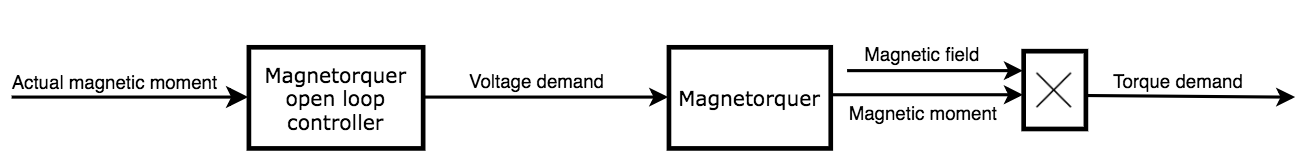
\includegraphics[width=1\linewidth]{figures/MT_open_loop}
	\caption{Magnetorquer open loop control }
	\label{fig:op}
\end{figure}

\subsection{Relation between the coil current and generated magnetic field} 
The knowledge about the relation between coil current and generated magnetic field in any given point in space, can be used for fault detection. The magnetic field in the center of a square coil is computed using the law of Biot-Savart \cite{SJ}:
\begin{flalign}
	d\vec B_{mt} = \frac{\mu_0 I}{4 \pi}  \frac{d \vec s \times \hat{\vec r}}{r^2}
	\label{eq:BS}
\end{flalign} 
where \\
$\vec B_{mt}$ is the magnetic field generated by magnetorquer \\
$\mu_0$ is a constant called permeability of free space and is equal with $4\pi \times 10^{-7}  \ Tm/A$ \\
$I$ is the current \\
$d \vec s $ is a length element in the direction of current \\
$\hat{\vec r}$ is the direction from $d \vec s$ to a particular position \\
$r$ is the distance from $d \vec s$ to a particular position

Equation \ref{eq:BS} represents an infinitesimal element, thus integrating the equation over the whole coil gives the generated magnetic field.
